\documentclass[aspectratio=1610,t]{beamer}

\author{Mihai Lefter}
\title{Python Programming}
\providecommand{\mySubTitle}{Flow Control}
\providecommand{\myConference}{Programming Course}
\providecommand{\myDate}{26-11-2019}
\providecommand{\myGroup}{}
\providecommand{\myDepartment}{}
\providecommand{\myCenter}{}

\usetheme{lumc}

\usepackage{minted}
\usepackage{tikz}
\usepackage[many]{tcolorbox}

\definecolor{monokaibg}{HTML}{272822}
\definecolor{emailc}{HTML}{1e90FF}
\definecolor{scriptback}{HTML}{CDECF0}
\definecolor{ipyout}{HTML}{F0FFF0}

\newenvironment{ipython}
 {\begin{tcolorbox}[title=IPython,
                   title filled=false,
                   fonttitle=\scriptsize,
                   fontupper=\footnotesize,
                   enhanced,
                   colback=monokaibg,
                   drop small lifted shadow,
                   boxrule=0.1mm,
                   left=0.1cm,
                   arc=0mm,
                   colframe=black]}
 {\end{tcolorbox}}



\newenvironment{terminal}
 {\begin{tcolorbox}[title=terminal,
                   title filled=false,
                   fonttitle=\scriptsize,
                   fontupper=\footnotesize,
                   enhanced,
                   colback=monokaibg,
                   drop small lifted shadow,
                   boxrule=0.1mm,
                   left=0.1cm,
                   arc=0mm,
                   colframe=black]}
 {\end{tcolorbox}}


\newcommand{\hrefcc}[2]{\textcolor{#1}{\href{#2}{#2}}}
\newcommand{\hrefc}[3]{\textcolor{#1}{\href{#2}{#3}}}

\newcounter{cntr}
\renewcommand{\thecntr}{\texttt{[\arabic{cntr}]}}

\newenvironment{pythonin}[1]
{\VerbatimEnvironment
  \begin{minipage}[t]{0.11\linewidth}
   \textcolor{green}{\texttt{{\refstepcounter{cntr}In \thecntr:}}}
  \end{minipage}%
  \begin{minipage}[t]{0.89\linewidth}%
  \begin{minted}[
    breaklines=true,style=monokai]{#1}}
 {\end{minted}
 \end{minipage}}

\newenvironment{pythonout}
{%
  \addtocounter{cntr}{-1}
  \begin{minipage}[t]{0.11\linewidth}
   \textcolor{red}{\texttt{{\refstepcounter{cntr}Out\thecntr:}}}
  \end{minipage}%
  \color{ipyout}%
  \ttfamily%
  \begin{minipage}[t]{0.89\linewidth}%
}
{\end{minipage}}

\newenvironment{pythonerr}[1]
{\VerbatimEnvironment
  \begin{minted}[
    breaklines=true,style=monokai]{#1}}
 {\end{minted}}


\newenvironment{pythonfile}[1]
 {\begin{tcolorbox}[title=#1,
                    title filled=false,
                    coltitle=LUMCDonkerblauw,
                    fonttitle=\scriptsize,
                    fontupper=\footnotesize,
                    enhanced,
                    drop small lifted shadow,
                    boxrule=0.1mm,
                    leftrule=5mm,
                    rulecolor=white,
                    left=0.1cm,
                    colback=white!92!black,
                    colframe=scriptback]}
 {\end{tcolorbox}}


\newenvironment{pythoncode}
 {\begin{tcolorbox}[title filled=false,
                    coltitle=LUMCDonkerblauw,
                    fonttitle=\scriptsize,
                    fontupper=\footnotesize,
                    enhanced,
                    drop small lifted shadow,
                    boxrule=0.1mm,
                    leftrule=5mm,
                    rulecolor=white,
                    left=0.1cm,
                    colback=white!92!black,
                    colframe=scriptback]}
 {\end{tcolorbox}}


\newenvironment{pythonoutnonumber}
{%
  \color{ipyout}%
  \ttfamily%
}
{}


\usepackage{booktabs}

\begin{document}

% This disables the \pause command, handy in the editing phase.
%\renewcommand{\pause}{}

% Make the title slide.
\makeTitleSlide{\includegraphics[height=3.5cm]{../../images/Python.pdf}}

% First page of the presentation.
\section{Introduction}
\makeTableOfContents


\section{Working with scripts}

\begin{pframe}
 Interpreters are great for prototyping, but not really suitable if you want to
 share or release code. To do so, we write our Python commands in scripts (and
 later, modules).

 A script is a simple text file containing Python instructions to execute.
\end{pframe}


\subsection{Executing scripts}
\begin{pframe}
 There are two common ways to execute a script:
  \begin{itemize}
   \item As an argument of the Python interpreter command.
   \item As a standalone executable (with the appropriate shebang line and
   file mode).
  \end{itemize}
  \medskip

  IPython gives you a third option:
  \begin{itemize}
   \item As an argument of the \texttt{\%run} magic.
  \end{itemize}
\end{pframe}


\subsection{Writing your script}
\begin{pframe}
 Let's start with a simple hello world example.\\

 Open your text editor and write the following Python statement:

 \begin{pythonfile}{first\_script.py}
  \begin{minted}[linenos]{python}
print("Hello world!")
  \end{minted}
 \end{pythonfile}
Save the file as first\_script.py and go to your shell.
\end{pframe}

\subsection{Running the script}
\begin{pframe}
 Let's try the first method, i.e., using your script as an argument:
 \begin{terminal}
  \color{white}{\texttt{\$ python first\_script.py}}
 \end{terminal}
  Is the output as you expect?
\end{pframe}

\begin{pframe}
  For the second method, we need to do two more things:
  \begin{itemize}
   \item Open the script in your editor and add the following line to the very
   top:
   \begin{itemize}
    \item \mintinline{python}{#!/usr/bin/env python}
   \end{itemize}
   \item Save the file, go back to the shell, and allow the file to be executed.
  \end{itemize}
 \begin{terminal}
  \color{white}{\texttt{\$ chmod +x first\_script.py}}
 \end{terminal}
You can now execute the file directly:
\begin{terminal}
  \color{white}{\texttt{\$ ./first\_script.py}}
 \end{terminal}
 Is the output the same as the previous method?
\end{pframe}

\begin{pframe}
 Finally, try out the third method. Open an IPython interpreter session and do:
 \begin{ipython}
  \begin{pythonin}{python}
%run first_script.py
  \end{pythonin}
 \end{ipython}
\end{pframe}


\section{Sequential Execution}

\begin{pframe}
 \begin{center}
   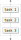
\includegraphics[width=0.25\textwidth]{../../images/flow_sequential.pdf}
 \end{center}
\end{pframe}

\begin{pframe}
 \begin{minipage}{0.37\textwidth}
 \begin{center}
   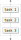
\includegraphics[width=0.50\textwidth]{../../images/flow_sequential.pdf}
 \end{center}
 \end{minipage}%
 \begin{minipage}{0.57\textwidth}
 \begin{pythonfile}{sum.py}
  \begin{minted}[linenos]{python}
a = 100
b = 200
print(a+b)
  \end{minted}
 \end{pythonfile}
 \begin{terminal}
  \color{white}{\texttt{\$ python sum.py \\
300}}
 \end{terminal}
 \end{minipage}
\end{pframe}

\subsection{Intermezzo - User input}
\begin{pframe}
Performed with the \emp{input([prompt])} built-in function:
 \begin{itemize}
  \item If the \emp{prompt} argument is present, it is written to the standard
        output.
  \item The user input is then read as a string.
 \end{itemize}
 \pause
 \begin{pythonfile}{sum.py}
  \begin{minted}[linenos]{python}
a = input('a = ')
b = input('b = ')
print(a+b)
  \end{minted}
 \end{pythonfile}
 \pause
 \begin{terminal}
  \color{white}{\texttt{\$ python sum.py \\
a = 100 \\
b = 200 \\
100200}}
 \end{terminal}
 \pause
 \begin{tikzpicture}[remember picture,overlay]
    \node[xshift=-6.5cm,yshift=-6.64cm] at (current page.north east)
    {
\includegraphics[width=5.8cm]{../../images/questions.pdf}};
 \end{tikzpicture}
\end{pframe}

\begin{pframe}
Performed with the \emp{input([prompt])} built-in function:
 \begin{itemize}
  \item If the \emp{prompt} argument is present, it is written to the standard
        output.
  \item The user input is then read as a \empt{string}.
 \end{itemize}
 \begin{pythonfile}{sum.py}
  \begin{minted}[linenos]{python}
a = int(input('a = '))
b = int(input('b = '))
print(a+b)
  \end{minted}
 \end{pythonfile}
 \begin{terminal}
  \color{white}{\texttt{\$ python sum.py \\
a = 100 \\
b = 200 \\
300}}
 \end{terminal}
\end{pframe}


\section{Conditionals}
\begin{pframe}
 \begin{center}
   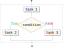
\includegraphics[width=0.55\textwidth]{../../images/flow_conditional.pdf}
 \end{center}
\end{pframe}

\begin{pframe}
 \begin{center}
   \includegraphics[width=0.55\textwidth]{../../images/flow_conditional_if_only.pdf}
 \end{center}
\end{pframe}

\begin{pframe}
 \begin{center}
   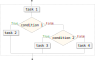
\includegraphics[width=0.75\textwidth]{../../images/flow_conditional_chained_if.pdf}
 \end{center}
\end{pframe}

\subsection{Truth Value Testing}
\begin{pframe}
%  Any object can be tested for its \textbf{truth} value:
 \begin{itemize}
 \item Built-in objects considered \textcolor{red}{false}:
 \begin{itemize}
   \item constants defined to be \textcolor{red}{false}: \emp{None} and \emp{False}.
   \pause
   \item zero of any numeric type: \emp{0}, \emp{0.0}, \emp{0j},
         \emp{Decimal(0)}, \emp{Fraction(0, 1)}.
   \pause
   \item empty sequences and collections: \emp{''}, \emp{()}, \emp{[]},
         \emp{\{\}}, \emp{set()}, \emp{range(0)}.
  \end{itemize}
  \pause
  \item For the moment, let's assume that any other object is considered
  \textcolor{green}{true}.
 \end{itemize}
 \pause
 \begin{ipython}
  \begin{pythonin}{python}
bool(0)
  \end{pythonin}
  \begin{pythonout}
False
  \end{pythonout}\\ \\
  \begin{pythonin}{python}
bool(1)
  \end{pythonin}
  \begin{pythonout}
True
  \end{pythonout}\\ \\
  \begin{pythonin}{python}
bool([False])
  \end{pythonin}
  \begin{pythonout}
True
  \end{pythonout}
 \end{ipython}
\end{pframe}

\subsection{Comparisons}
\begin{pframe}
\begin{table}[]
\begin{tabular}{@{}lll@{}}
\toprule
  Operation    & Meaning & Example \\ \toprule
  \emp{<}      & strictly less than & \pythoninline{x < y} \\
  \emp{<=}     & less than or equal & \pythoninline{x <= y} \\
  \emp{>}      & strictly greater than & \pythoninline{x > y} \\
  \emp{>=}     & greater than or equal & \pythoninline{x >= y} \\
  \emp{==}     & equal & \pythoninline{x == y} \\
  \emp{!=}     & not equal & \pythoninline{x != y} \\ \midrule
  \emp{is}     & object identity & \pythoninline{x is y} \\
  \emp{is not} & negated object identity & \pythoninline{x is not y} \\ \bottomrule
\end{tabular}
\end{table}
\end{pframe}

\begin{pframe}
 \begin{ipython}
  \begin{pythonin}{python}
3 < 4
  \end{pythonin}
  \begin{pythonout}
True
  \end{pythonout} \\ \\
  \begin{pythonin}{python}
3 <= 3.5
  \end{pythonin}
  \begin{pythonout}
True
  \end{pythonout} \\ \\
  \begin{pythonin}{python}
3 == 3.0
  \end{pythonin}
  \begin{pythonout}
True
  \end{pythonout}
 \\ \\
  \begin{pythonin}{python}
3 is 3.0
  \end{pythonin}
  \begin{pythonout}
False
  \end{pythonout} \\ \\
  \begin{pythonin}{python}
3 is 3
  \end{pythonin}
  \begin{pythonout}
True
  \end{pythonout}
 \end{ipython}
\end{pframe}


\subsection{Boolean (Logical) Operations}
\begin{pframe}
\begin{table}[]
\begin{tabular}{@{}llc@{}}
\toprule
 Operation     & Result & Notes \\ \midrule
 \pythoninline{x or y}  & if \emp{x} is false, then \emp{y}, else \emp{x} & (1) \\
 \pythoninline{x and y} & if \emp{x} is false, then \emp{x}, else \emp{y} & (2) \\
 \pythoninline{not x}   & if \emp{x} is false, then \emp{True}, else \emp{False} & (3) \\ \bottomrule
\end{tabular}
\end{table}
 \begin{enumerate}
  \item It evaluates \emp{y} only if \emp{x} is false.
  \item It evaluates \emp{y} only if \emp{x} is true.
  \item \pythoninline{not x == y} is interpreted as \pythoninline{not (x == y)}
  and \pythoninline{x == not y} is a syntax error.
 \end{enumerate}
\end{pframe}

\begin{pframe}
\begin{table}[]
\begin{tabular}{@{}cc|cc@{}}
\toprule
  \emp{x}     & \emp{y}     & \emp{x or y} & \emp{x and y} \\ \midrule
  \emp{True}  & \emp{True}  & \emp{True}   & \emp{True}    \\
  \emp{True}  & \emp{False} & \emp{True}   & \emp{False}   \\
  \emp{False} & \emp{True}  & \emp{True}   & \emp{False}   \\
  \emp{False} & \emp{False} & \emp{False}   & \emp{False}  \\ \bottomrule
\end{tabular}
\end{table}
\end{pframe}

\begin{pframe}
 \begin{ipython}
  \begin{pythonin}{python}
3 < 4 and 5 <= 10
  \end{pythonin}
  \begin{pythonout}
True
  \end{pythonout} \\ \\
  \begin{pythonin}{python}
3 < 4 or 5 <= 10
  \end{pythonin}
  \begin{pythonout}
True
  \end{pythonout} \\ \\
  \begin{pythonin}{python}
3 < 4 and 5 > 10
  \end{pythonin}
  \begin{pythonout}
False
  \end{pythonout}
 \\ \\
  \begin{pythonin}{python}
3 < 4 and 5 > 10
  \end{pythonin}
  \begin{pythonout}
True
  \end{pythonout}
 \end{ipython}
\end{pframe}

\subsection{\emp{if} statement}
\begin{pframe}
 \begin{minipage}{0.47\textwidth}
 \begin{center}
   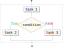
\includegraphics[width=0.80\textwidth]{../../images/flow_conditional.pdf}
 \end{center}
 \end{minipage}%
 \begin{minipage}{0.47\textwidth}
 \begin{pythonfile}{max.py}
  \begin{minted}[linenos]{python}
a = int(input('a = '))
b = int(input('b = '))

if a > b:
    print(a)
else:
    print(b)
  \end{minted}
 \end{pythonfile}

 \begin{terminal}
  \color{white}{\texttt{\$ python max.py \\
a = 100 \\
b = 200 \\
200}}
 \end{terminal}
 \end{minipage}
\end{pframe}

\begin{pframe}
 \begin{minipage}{0.57\textwidth}
 \begin{center}
   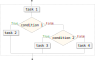
\includegraphics[width=0.90\textwidth]{../../images/flow_conditional_chained_if.pdf}
 \end{center}
 \end{minipage}%
 \begin{minipage}{0.37\textwidth}
 \begin{pythonfile}{compare.py}
  \begin{minted}[linenos]{python}
a = int(input('a = '))
b = int(input('b = '))

if a > b:
    print(a)
elif a == b:
    print('equal')
else:
    print(b)
  \end{minted}
 \end{pythonfile}

 \begin{terminal}
  \color{white}{\texttt{\$ python compare.py \\
a = 100 \\
b = 100 \\
equal}}
 \end{terminal}
 \end{minipage}
\end{pframe}

\section{Indentation}
\begin{pframe}
 Python uses indentation to delimit blocks
 \begin{itemize}
   \item Instead of \emp{begin ... end} or \emp{\{ ... \}} in other languages.
   \item Always increase indentation by 4 spaces, never use tabs.
   \begin{itemize}
     \item In any case, be consistent.
   \end{itemize}
 \end{itemize}
 \begin{pythonfile}{indentation\_example.py}
  \begin{minted}[linenos]{python}
if False:
    if False:
        print('Why am I here?')
    else:
        while True:
            print('When will it stop?')
    print("And we're back to the first indentation level")
  \end{minted}
 \end{pythonfile}
\end{pframe}



\section{Loops}
\begin{pframe}
 \begin{center}
   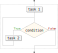
\includegraphics[width=0.50\textwidth]{../../images/flow_loops.pdf}
 \end{center}
\end{pframe}



\subsection{\pythoninline{while} statement}
\begin{pframe}
 \begin{minipage}{0.47\textwidth}
 \begin{center}
   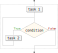
\includegraphics[width=0.80\textwidth]{../../images/flow_loops.pdf}
 \end{center}
 \end{minipage}%
 \begin{minipage}{0.47\textwidth}
 \begin{pythonfile}{while\_example.py}
  \begin{minted}[linenos]{python}
i = 0
while i < 5:
    print(i)
    i += 1
  \end{minted}
 \end{pythonfile}

 \begin{terminal}
  \color{white}{\texttt{\$ python while\_example.py \\
0\\
1\\
2\\
3\\
4\\}}
 \end{terminal}
 \end{minipage}

\end{pframe}

\subsection{\pythoninline{for} statement}
\begin{pframe}
 Used to iterate over a sequence.
 \begin{pythonfile}{for\_example.py}
  \begin{minted}[linenos]{python}
colors = ['red', 'white', 'blue', 'orange']

for color in colors:
    print(color)
  \end{minted}
 \end{pythonfile}
 \pause
 \begin{terminal}
  \color{white}{\texttt{\$ python for\_example.py\\
red\\
white\\
blue\\
orange\\
}}
 \end{terminal}
\end{pframe}


\subsection{Python anti-patterns}
\begin{pframe}
These are common for programmers coming from other languages.
 \begin{pythonfile}{unpythonic.py}
  \begin{minted}[linenos]{python}
i = 0
while i < len(colors):
    print(colors[i])
    i += 1

for i in range(len(colors)):
    print(colors[i])
  \end{minted}
 \end{pythonfile}

We call them unpythonic.
\end{pframe}


\subsection{Additionals}
\begin{pframe}
 \begin{pythonfile}{iteration.py}
  \begin{minted}[linenos]{python}
# Iteration with values and indices:
for i, color in enumerate(['red', 'yellow', 'blue']):
    print(i, '->', color)

# Taking two sequences together:
for city, population in zip(['Delft', 'Leiden'], [101030, 121562]):
    print(city, '->', population)

# Iterating over a dictionary yields keys:
for key in {'a': 33, 'b': 17, 'c': 18}:
    print(key)

# Iterating over a file yields lines:
for line in open('data/short_file.txt'):
    print(line)
  \end{minted}
 \end{pythonfile}
\end{pframe}


\section{Extras}

\subsection{The pass statement}
\begin{pframe}
 If you ever need a statement syntactically but don't want to do anything, use \texttt{pass}.
 \begin{pythonfile}{comments\_example.py}
  \begin{minted}[linenos]{python}
while False:
    # This is never executed anyway.
    pass
  \end{minted}
 \end{pythonfile}
\end{pframe}

\subsection{Comments}
\begin{pframe}
 Comments are prepended by \texttt{\#} and completely ignored.
 \begin{pythonfile}{comments\_example.py}
  \begin{minted}[linenos]{python}
# Create the list.
l = []

# Add 42 to this list.
l.append(42)
  \end{minted}
 \end{pythonfile}
\end{pframe}

\section{Hands on!}
\begin{pframe}
 \vspace{-0.5cm}
 \begin{enumerate}
  \item Write a program that prints those numbers which are divisible by
  13 and multiple of 5, between 10 and 1313 (both included).
 \end{enumerate}
\end{pframe}


\end{document}
